% Created 2017-11-27 Mon 14:25
% Intended LaTeX compiler: pdflatex
\documentclass[11pt]{article}
\usepackage[utf8]{inputenc}
\usepackage{lmodern}
\usepackage[T1]{fontenc}
\usepackage{fixltx2e}
\usepackage{graphicx}
\usepackage{longtable}
\usepackage{float}
\usepackage{wrapfig}
\usepackage{rotating}
\usepackage[normalem]{ulem}
\usepackage{amsmath}
\usepackage{textcomp}
\usepackage{marvosym}
\usepackage{wasysym}
\usepackage{amssymb}
\usepackage{amsmath}
\usepackage[version=3]{mhchem}
\usepackage[numbers,super,sort&compress]{natbib}
\usepackage{natmove}
\usepackage{url}
\usepackage{minted}
\usepackage{underscore}
\usepackage[linktocpage,pdfstartview=FitH,colorlinks,
linkcolor=blue,anchorcolor=blue,
citecolor=blue,filecolor=blue,menucolor=blue,urlcolor=blue]{hyperref}
\usepackage{attachfile}
\usepackage[left=1in, right=1in, top=1in, bottom=1in, nohead]{geometry}
\usepackage{fancyhdr}
\usepackage{hyperref}
\usepackage{setspace}
\usepackage[labelfont=bf]{caption}
\usepackage{amsmath}
\usepackage{enumerate}
\usepackage[parfill]{parskip}
\usepackage[version=3]{mhchem}
\date{Due: November 2017}
\title{}
\begin{document}

\title{Homework 4\\Lectures 5: Potential Energy Sufaces\\(CBE 60547)}
\author{Jeonghyun Ko, Gray Laughlin, Yujia Wang}
\maketitle

In this assignment you will determine some of the properties of \textbf{acetaldehyde} (\ce{CH3CHO}), its isomer \textbf{vinyl alcohol} (\ce{H2C=CH(OH)}), and the \textbf{transtion state} (TS) that interconverts the two:

\begin{center}
\begin{center}

\includegraphics[width=.9\linewidth]{fig1.png}
\end{center}
\end{center}



\section{Characterizing the reactant and product}
\label{sec:org04e2a95}
\begin{enumerate}[(a)]
\item First, optimize the structures of the reactant acetaldehyde and product vinyl alcohol at the Hartree-Fock level with the 6-31G(d) basis set. Make a table of the key internal coordinates in the two (note you will figure out the TS below):
\end{enumerate}

\begin{center}
\begin{tabular}{lrlr}
\hline
 & Acetaldehyde & Transition State & Vinyl alcohol\\
\hline
H\(_{\text{1}}\)–C (\AA{}) & 1.08 & -- & 2.47\\
C–C (\AA{}) & 1.50 & -- & 1.32\\
C–O (\AA{}) & 1.19 & -- & 1.35\\
O-H\(_{\text{1}}\) (\AA{}) & 2.55 & -- & 0.95\\
\hline
\end{tabular}
\end{center}

\begin{enumerate}[(b)]
\item Which geometry optimization method did you use in (a)? What type of coordinate system? What were the convergence criteria?
\end{enumerate}
\linebreak
The Quasi-Newton Raphson method with BFGS Hessian updates was used to optimize the geometry of the molecules. Coordinates were described in a Z-matrix format. Optimization convergence was reached when the density matrix update was less than 1E-5.   

\begin{enumerate}[(c)]
\item Calculate the vibrational spectra of the reactant and product. Confirm that both are true minima (if not, adjust and recalculate). Identify the most prominent (intense) infrared vibrational modes in the two. Could you distinguish these two by their vibrational spectra?
\end{enumerate}
\linebreak

The vibrational frequencies are different for the two molecules. The most prominent frequencies are 2032 cm\(^{\text{-1}}\) and 1233.84 cm\(^{\text{-1}}\) for the reactant and product respectively. The spectra are easily distinguishable. 

Reactant IR Spectra:

\begin{center}
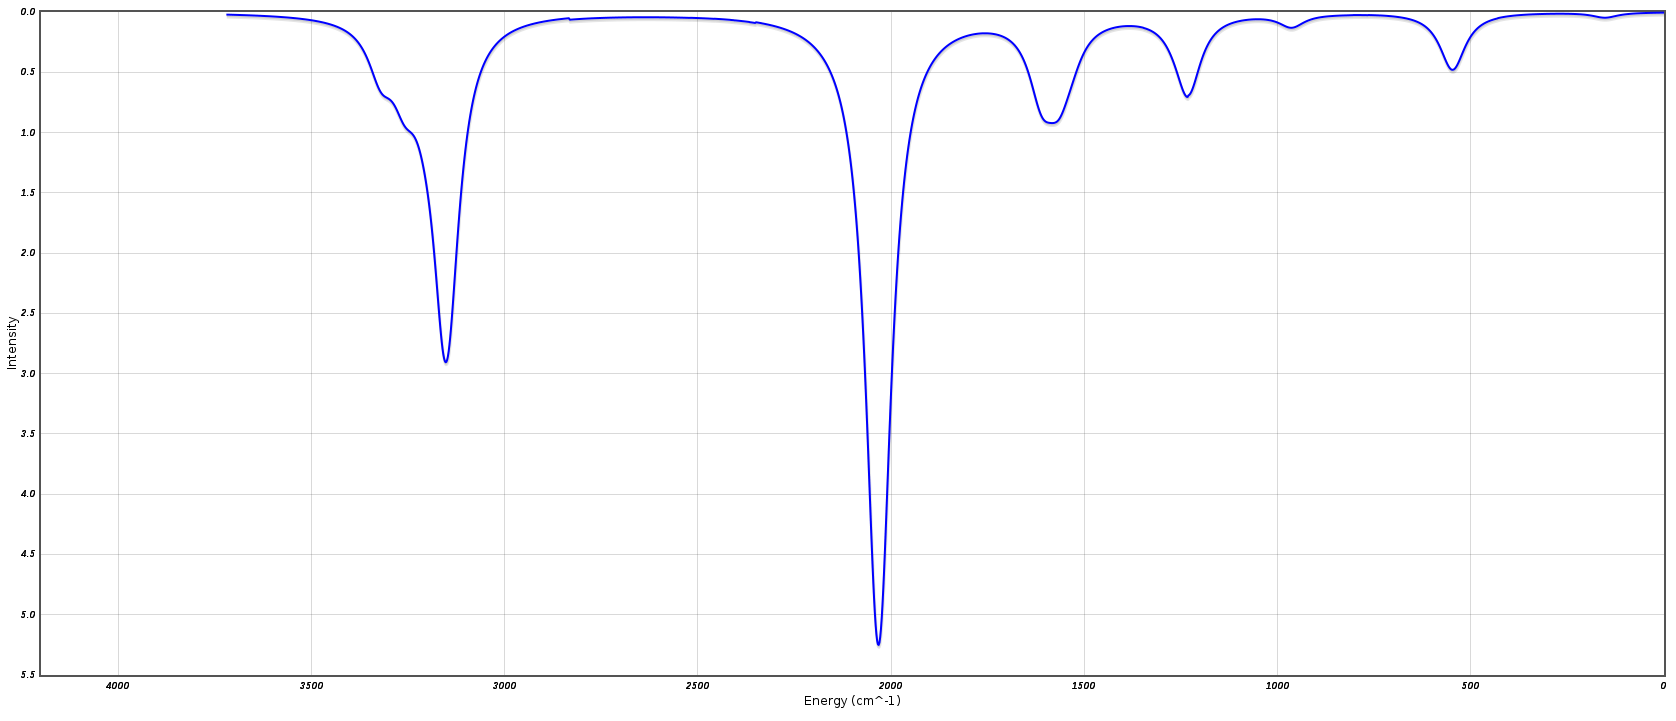
\includegraphics[width=.9\linewidth]{./plotreact.png}
\end{center}

Product IR Spectra:

\begin{center}
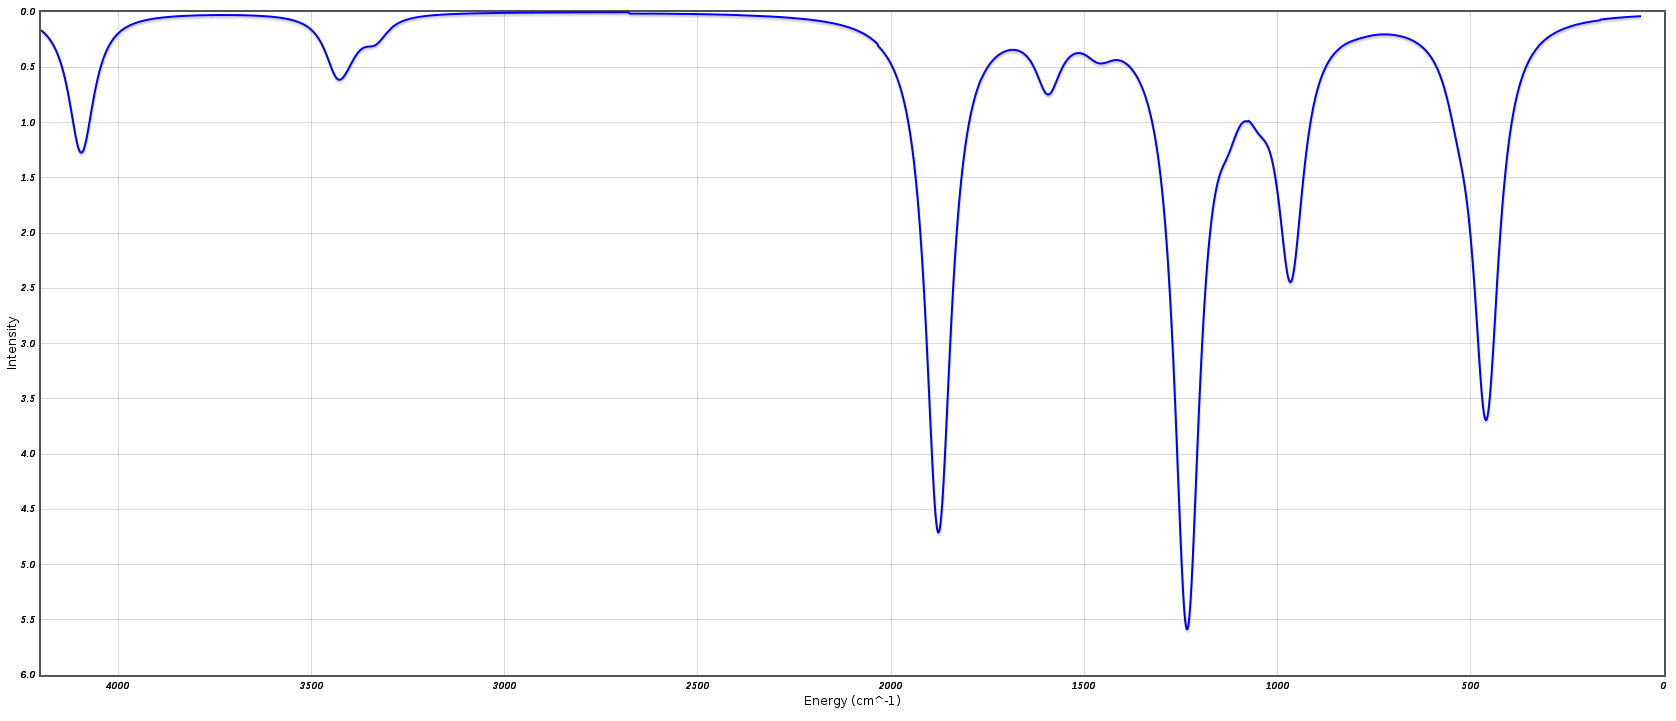
\includegraphics[width=.9\linewidth]{./plotprod.png}
\end{center}

\begin{enumerate}[(d)]
\item Perform single-point energy calculations on the reactant and product at the MP2/6-31G(d) level.  Use the results to complete the table below:
\end{enumerate}

\begin{center}
\begin{tabular}{lrr}
\hline
 & Product \(-\) reactant  (kJ/mol) & TS \(-\) reactant (kJ/mol)\\
\hline
HF/6-31G(d) & 71.09 & 368.44\\
MP2/6-31G(d) & 70.89 & 309.72\\
ZPE & 3.0 & -12.01\\
MP2 + ZPE & 73.89 & 297.71\\
\hline
\end{tabular}
\end{center}
react HF = -152.9159655 hart
prod HF = -152.888888 hart 

prod MP2 = -153.32002 hart 
react MP2 = -153.34692 hart

prod ZPE = 160.4 kJ/mol
react ZPE = 157.4 kJ/mol

\begin{enumerate}[(e)]
\item From the frequency calculations on the reactant and product, extract \(H^{\circ}(298)-H(0)\) for each.  Combine with the MP2 + ZPE results to estimate the 298 K reaction enthalpy.
\end{enumerate}

Heat capacity functions of T:
Cp(reactant) = 0.0772T + 31.832 
Cp(product) = 0.0722T + 30.553


\begin{center}
\begin{tabular}{lrrr}
 & Reactant (kJ/mol) & Product (kJ/mol) & Rxn  (kJ/mol)\\
H(0) & -402612 & -402541 & 71\\
Integrated Heat Cap. & 12904.9 & 12794 & --\\
H\(^{\^{}}\)(298) & -389707.1 & -389747.4 & -40.3\\
\end{tabular}
\end{center}


\section{Transition state by scanning}
\label{sec:orga59738f}
\begin{enumerate}[(a)]
\item Do a rigid scan about the H\(_{\text{1}}\)-C-C-O dihedral in acetaldehyde. It is easiest to do this using a z-matrix representation of acetaldehyde. Construct a z-matrix based on your optimized acetaldehyde structure and do a series of energy evaluations as you vary the dihedral angle. Approximately how large is the barrier to rotation about the C–C bond, in kJ/mol?
\end{enumerate}

All single-point energy calculations performed in Orca using the MP2 method. The rotation barrier is approximately 4.6 kJ/mol.

\begin{center}
\label{energies}
\begin{tabular}{rr}
0 & -153.2561\\
36 & -153.2548\\
72 & -153.2544\\
108 & -153.2560\\
144 & -153.2554\\
180 & -153.2542\\
216 & -153.2556\\
252 & -153.2559\\
288 & -153.2542\\
324 & -153.2549\\
360 & -153.2561\\
\end{tabular}
\end{center}


\begin{minted}[frame=lines,fontsize=\scriptsize,linenos]{python}
import matplotlib.pyplot as plt

dihedrals = [entry[0] for entry in table]
energies = [entry[1] for entry in table]


plt.plot(dihedrals, energies, 'b', label='Energy Scan')
#,spline1,Rxn_label,spline2)
plt.xticks(dihedrals)
plt.xlabel('Dihedral Angle (Degrees)')
plt.ylabel('Energy (Hartrees)')
plt.legend(loc='best')
plt.tight_layout()
plt.savefig('./energy_scan.png')
plt.show()
\end{minted}

\begin{center}
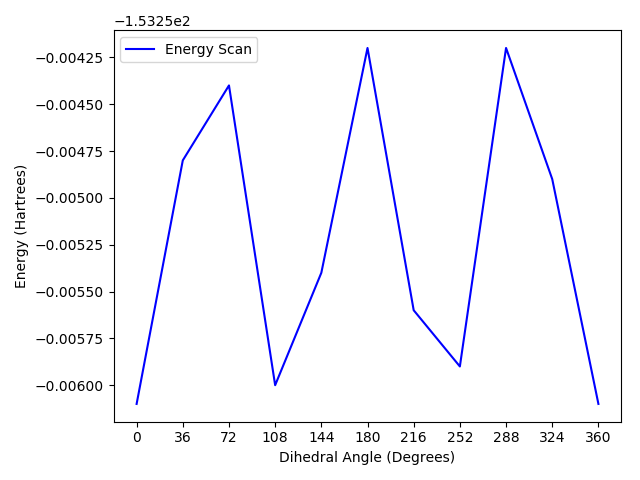
\includegraphics[width=.9\linewidth]{./energyscan.png}
\end{center}

\section{Transition state optimization}
\label{sec:org18fbbb7}
\begin{enumerate}[(a)]
\item Guess a structure near the transition state that connects acetaldehyde to vinyl alcohol (note I gave you some hints in the figure) and compute the Hessian at the HF/6-31G(d) level to make sure you are near a saddle point.  Once you have a satisfactory guess, search from this starting point for the transition state. Make sure your calculation converges, and calculate the vibrational spectrum again to make sure you landed at the saddle point. Add the key internal coordinates to the Table in 1(a).

\item What is the magnitude of the imaginary vibrational mode at the transition state?

\item Perform a single-point MP2/6-31G(d) calculations on this transition state. Add the results to the Table in 1(c).

\item Use transition state theory to estimate the rate constant for this reaction at 298 K.  From the frequency calculations on the reactant and transition state, extract \(G^{\circ}(298 K)- G( K)\) for each.  Combine these results with the MP2 + ZPE energies to estimate \(\Delta G^{\ddagger}(298)\).  Evaluate the rate constant using the TST expression:
\end{enumerate}

\begin{equation}
 k(T) =\frac{k_{B} T}{h} e^{-\Delta G^{\ddagger}(T)/k_{B}T}
\end{equation}


\subsection{Solution}
\label{sec:orgd3cf470}

\subsubsection{a)}
\label{sec:orgcdf6627}

Input file of GAMESS for TS structure guess
\begin{minted}[frame=lines,fontsize=\scriptsize,linenos]{sh}
 $CONTRL SCFTYP=RHF RUNTYP=HESSIAN 
       ICHARG=0 MULT=1 COORD=ZMTMPC $END
 $BASIS GBASIS=N31 NGAUSS=6 NDFUNC=1 $END
 $DATA
C2H4O
C1 1
C 0.0000000 0 0.0000000 0 0.0000000 0 0 0 0
C 1.5400000 1 0.0000000 0 0.0000000 0 1 0 0
O 1.2750000 1 120.00000 1 0.0000000 0 2 1 0
H 1.0900000 1 117.38979 1 -161.69239 1 2 1 3
H 1.0900000 1 109.47122 1 -110.00000 1 1 2 3
H 1.5049141 1 69.873799 1 -11.355914 1 1 2 3
H 1.0900000 1 109.47122 1 130.00000 1 1 2 3
 $END
\end{minted}

\(\vspace{3pt}\)

The vibrational modes for the guessed TS structure

\begin{center}
\begin{tabular}{rr}
Mode & Frequency (cm\(^{-1}\))\\
\hline
1 & 1170.63841 I\\
2 & 220.80887\\
3 & 0.01753\\
4 & 0.00648\\
5 & 0.00508\\
6 & 232.68365\\
7 & 382.62252\\
8 & 531.21061\\
9 & 708.46004\\
10 & 822.0281\\
11 & 952.78115\\
12 & 1193.26027\\
13 & 1274.08053\\
14 & 1335.08057\\
15 & 1398.97709\\
16 & 1504.56455\\
17 & 1570.71896\\
18 & 1722.9671\\
19 & 3196.77908\\
20 & 3228.2914\\
21 & 3262.89519\\
\end{tabular}
\end{center}

\(\vspace{3pt}\)

Input file of GAMESS for finding TS structure
\begin{minted}[frame=lines,fontsize=\scriptsize,linenos]{sh}
 $CONTRL SCFTYP=RHF RUNTYP=SADPOINT 
       ICHARG=0 MULT=1 COORD=ZMTMPC $END
 $BASIS GBASIS=N31 NGAUSS=6 NDFUNC=1 $END
 $STATPT HESS=CALC NSTEP=100 $END
 $DATA
C2H4O
C1 1
C 0.0000000 0 0.0000000 0 0.0000000 0 0 0 0
C 1.5399999 1 0.0000000 0 0.0000000 0 1 0 0
O 1.2750004 1 120.00001 1 0.0000000 0 2 1 0
H 1.0899999 1 117.38978 1 -161.69236 1 2 1 3
H 1.0899999 1 109.47118 1 -109.99999 1 1 2 3
H 1.5049143 1 69.873796 1 -11.355956 1 1 2 3
H 1.0900000 1 109.47123 1 129.99998 1 1 2 3
 $END
\end{minted}


Then, perform a single-point calculation to confirm the vibrational modes of converged structure

\(\vspace{3pt}\)

Input file of GAMESS for finding TS structure
\begin{minted}[frame=lines,fontsize=\scriptsize,linenos]{sh}
 $CONTRL SCFTYP=RHF RUNTYP=HESSIAN 
       ICHARG=0 MULT=1 COORD=ZMTMPC $END
 $BASIS GBASIS=N31 NGAUSS=6 NDFUNC=1 $END
 $DATA
C2H4O
C1 1
C 0.0000000 0 0.0000000 0 0.0000000 0 0 0 0
C 1.4205123 1 0.0000000 0 0.0000000 0 1 0 0
O 1.2517072 1 109.17749 1 0.0000000 0 2 1 0
H 1.0807165 1 131.54793 1 -177.24197 1 2 1 3
H 1.0846693 1 110.03343 1 -73.713743 1 1 2 3
H 1.5184653 1 65.616181 1 7.9326391 1 1 2 3
H 1.0785697 1 120.71715 1 152.43909 1 1 2 3
 $END
\end{minted}

\(\vspace{3pt}\)

\begin{center}
\begin{tabular}{rr}
Mode & Frequency (cm\(^{-1}\))\\
\hline
1 & 2573.824 I\\
2 & 4.724\\
3 & 3.454\\
4 & 3.069\\
5 & 0.034\\
6 & 0.347\\
7 & 0.461\\
8 & 541.747\\
9 & 719.07\\
10 & 896.329\\
11 & 1078.011\\
12 & 1161.812\\
13 & 1270.518\\
14 & 1312.98\\
15 & 1432.017\\
16 & 1613.097\\
17 & 1729.381\\
18 & 2088.627\\
19 & 3254.42\\
20 & 3339.587\\
21 & 3357.344\\
\end{tabular}
\end{center}

\(\vspace{3pt}\)

The key internal coordinates
\begin{center}
\begin{tabular}{llrl}
 & Acetaldehyde & Transition State & Vinyl alcohol\\
\hline
\(H_{1}-C\) (\(\AA\)) &  & 1.51846 & \\
\(C-C\) (\(\AA\)) &  & 1.42051 & \\
\(C-O\) (\(\AA\)) &  & 1.25171 & \\
\(O-H_{1}\) (\(\AA\)) &  & 1.23416 & \\
\end{tabular}
\end{center}


\subsubsection{b)}
\label{sec:org73876c2}
The magnitude of the imaginary vibrational mode at the transition state is 2573.824.


\subsubsection{c)}
\label{sec:orga4d6157}
Input file of GAMESS for single-point MP2/6-31G(d) calculations on the transition state

\begin{minted}[frame=lines,fontsize=\scriptsize,linenos]{sh}
 $CONTRL SCFTYP=RHF MPLEVL=2 RUNTYP=ENERGY 
       ICHARG=0 MULT=1 COORD=ZMTMPC $END
 $BASIS GBASIS=N31 NGAUSS=6 NDFUNC=1 $END
 $DATA
C2H4O
C1 1
C 0.0000000 0 0.0000000 0 0.0000000 0 0 0 0
C 1.4205115 1 0.0000000 0 0.0000000 0 1 0 0
O 1.2517074 1 109.17751 1 0.0000000 0 2 1 0
H 1.0807169 1 131.54793 1 -177.24200 1 2 1 3
H 1.0846694 1 110.03348 1 -73.713741 1 1 2 3
H 1.5184649 1 65.616187 1 7.9326351 1 1 2 3
H 1.0785700 1 120.71714 1 152.43909 1 1 2 3
 $END
\end{minted}

\(\vspace{3pt}\)

\begin{center}
\begin{tabular}{lll}
 & Product - reactant (kJ/mol) & TS - reactant (kJ/mol)\\
\hline
HF/6-31G(d) &  & (-397204) - (-397582) = 377.3846\\
MP2/6-31G(d) &  & (-402285) - (-402606) = 321.1754\\
ZPE &  & (142.325482) - (157.354624) = -15.0291\\
MP2 + ZPE &  & 306.1463\\
\end{tabular}
\end{center}


\subsubsection{d)}
\label{sec:org86c7cc4}
Thermochemistry at T = 298.15 K

Using ideal gas, rigid rotor, harmonic normal mode approximations.\\


from the vibrational calculation of TS
\begin{minted}[frame=lines,fontsize=\scriptsize,linenos]{sh}
              E         H         G         CV        CP        S
           KJ/MOL    KJ/MOL    KJ/MOL   J/MOL-K   J/MOL-K   J/MOL-K
 ELEC.      0.000     0.000     0.000     0.000     0.000     0.000
 TRANS.     3.718     6.197   -40.298    12.472    20.786   155.948
 ROT.       3.718     3.718   -23.019    12.472    12.472    89.678
 VIB.     143.472   143.472   141.989    14.551    14.551     4.975
 TOTAL    150.909   153.388    78.671    39.495    47.809   250.601
\end{minted}

\(\vspace{3pt}\)
from the vibrational calculation of reactant
\begin{minted}[frame=lines,fontsize=\scriptsize,linenos]{sh}
              E         H         G         CV        CP        S
           KJ/MOL    KJ/MOL    KJ/MOL   J/MOL-K   J/MOL-K   J/MOL-K
 ELEC.      0.000     0.000     0.000     0.000     0.000     0.000
 TRANS.     3.718     6.197   -40.298    12.472    20.786   155.948
 ROT.       3.718     3.718   -23.218    12.472    12.472    90.347
 VIB.     159.926   159.926   155.471    19.320    19.320    14.943
 TOTAL    167.363   169.842    91.954    44.263    52.577   261.237
\end{minted}

\(\vspace{3pt}\)

Thus, we can compute \(\Delta G^{\ddagger}\) 

\begin{center}
\begin{tabular}{ll}
Compound & (MP2 + ZPE) + G\(_{corr}\) (kJ/mol)\\
\hline
TS - reactant & (306.1463) + (78.671 - 91.954) = 292.8633\\
\end{tabular}
\end{center}

\(\vspace{3pt}\)

$$ k(T) = \frac{k_{B} T}{h} e^{-\Delta G(T)^{\ddagger} / k_{B}T}  $$

$$ k(298 K) = \frac{(1.380662 \times 10^{-23})(298)}{6.626176 \times 10^{-34}} e^{\frac{-292.8633 \times 1000} {(8.314472) \times (298)}} = 2.88298 \times 10^{-39} s^{-1} $$




\section{Bronsted-Evans-Polanyi relations}
\label{sec:org1115fe2}

Your colleague wants to know if replacing one of the methyl H’s with an F will speed-up or slow down the isomerization. You know from experience that it is much easier to calculate relative rates than absolute ones.
\begin{enumerate}[(a)]
\item Perform additional calculations to determine whether the reaction is more or less exothermic with the F substituent.

\item Perform additional calculations to determine whether the reaction barrier is higher or lower with the F substituent.

\item Do your answers to (a) and (b) conform to expectations from the BEP relationship?
\end{enumerate}

\subsection{Solution}
\label{sec:orgdc02afd}

\subsubsection{a)}
\label{sec:orga95c7f9}

Using the same method as we used in the first three questions, we optimized the geometry of the reactant, the product and the transition state at the HF/6-31G(d) level, then calculated the single-point energies at the MP2/6-31G(d) level. Zero point energies were obtained from vibrational frequency calculations using the optimized geometries. All calculations were done using Gamess in WebMO. (1 Hartree = 2625.50 kJ/mol)

\begin{center}
\begin{tabular}{lrrrrr}
\hline
Energy (kJ/mol) & Reactant & Product & TS & TS - Reactant & Product - Reactant\\
\hline
HF/6-31G(d) & -660991 & -660925 & -660599 & 391.20 & 63.64\\
MP2/6-31G(d) & -662548 & -662492 & -662222 & 325.56 & 55.14\\
ZPE & 139.28 & 122.83 & 141.21 & 1.93 & -16.45\\
MP2 + ZPE & -662408 & -662370 & -662081 & 327.49 & 38.69\\
 &  &  &  &  & \\
\hline
\end{tabular}
\end{center}
Product - Reactant = 38.69 kJ/mol for F substituent.
Compared with the original reaction, the reaction with the F substituent is less exothermic.

\subsubsection{b)}
\label{sec:org4ea3194}

TS - Reactant = 327.49 kJ/mol for F substituent.
Compared with the original reaction, the reaction barrier with the F substituent is higher. 

\subsubsection{c)}
\label{sec:org7ff4914}

BEP relationship: the difference in activation energy between two reactions of the same family is proportional to the difference of their enthalpy of reaction.
Our answers to (a) and (b) conform to expectations from the BEP relationship.


\section{Useful Templates}
\label{sec:org1bd0899}

\subsection{Frequency calculation:}
\label{sec:orga69c24e}
\begin{verbatim}
$CONTRL SCFTYP=RHF RUNTYP=HESSIAN $END
$BASIS GBASIS=N31 NGAUSS=6 NDFUNC=1 $END
$FORCE METHOD=ANALYTIC VIBANL=.TRUE. $END
$GUESS GUESS=MOREAD NORB=xxx $END ! use if you have a converged SCF wavefunction to read in
$DATA
...
$END
\end{verbatim}


\subsection{Geometry optimization using redundant internal coordinates:}
\label{sec:org377c58c}
\begin{verbatim}
$CONTRL SCFTYP=RHF RUNTYP=OPTIMIZE NZVAR=”3n-6” $END
$BASIS GBASIS=N31 NGAUSS=6 NDFUNC=1 $END
$STATPT NSTEP=xx $END
$ZMAT DLC=.TRUE. AUTO=.TRUE. $END
$GUESS GUESS=MOREAD NORB=xxx $END ! use if you have a converged SCF wavefunction to read in
$DATA
 ...
$END
$VEC ! converged SCF wavefunction, if you have it
...
$END
\end{verbatim}


\subsection{Transition state search:}
\label{sec:org691aa53}
\begin{verbatim}
$CONTRL SCFTYP=RHF RUNTYP=SADPOINT NZVAR=”3n-6” $END
$BASIS GBASIS=N31 NGAUSS=6 NDFUNC=1 $END
$STATPT HESS=READ NSTEP=xx $END
$ZMAT DLC=.TRUE. AUTO=.TRUE. $END
$GUESS GUESS=MOREAD NORB=xxx $END ! use if you have a converged SCF wavefunction to read in
$DATA
...
$END
$HESS
...
$END
$VEC
...
$END
\end{verbatim}


\subsection{MP2 calculation:}
\label{sec:org55cbd2d}

\begin{verbatim}
$CONTRL SCFTYP=RHF RUNTYP=ENERGY MPLEVL=2 $END
$BASIS GBASIS=N31 NGAUSS=6 NDFUNC=1 $END
$DATA !
...
$END
\end{verbatim}


\subsection{CIS calculation:}
\label{sec:orge84e835}

\begin{verbatim}
$CONTRL SCFTYP=RHF RUNTYP=ENERGY CITYP=CIS $END
$BASIS GBASIS=N31 NGAUSS=6 NDFUNC=1 $END
$DATA !
...
$END
\end{verbatim}
\end{document}